\section{Global theory of plane curves}

The global theory is related to ``topology'' of the geometric objects.
For 1-dimensional geometry, i.e. curves, it's always oriented. And the simplest distinction in topology 
is ``open'' and ``closed''. 

\begin{definition}[Closed curves]
    \begin{itemize}\hfill
        \item We say 
        \(\alpha\colon I=[a,b]\to \mathbb{R}
        ^3\) 
        (or \(\mathbb{R}^2\)) 
        is a regular closed 
        curve, if 
        \(\alpha(a)=\alpha(b)\) 
        and 
        \(\alpha^{(k)}
        (a)=\alpha^{(k)}(b)\)
        (in another word, 
        \(\alpha\colon \mathbb{S}^1\to \mathbb{R}^3\) 
        is a differentiable curve).
        \item Furthermore, if 
        \(\alpha\) 
        has no 
        self-intersection point other than 
        $\alpha(a)=\alpha(b)$, 
        then we call $\alpha(s)$ to be a simple closed curve.
    \end{itemize}
\end{definition}
\begin{center}
    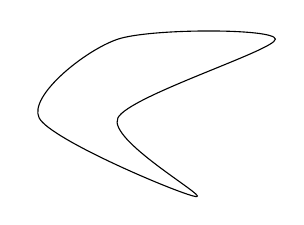
\begin{tikzpicture}
        \draw plot [smooth cycle] coordinates {(0,0) (1,1) (3,1) (1,0) (2,-1)};
    \end{tikzpicture}
\end{center}

\subsection{Isoperimetric inequality}
This is one of the oldest and most famous problem in geometry. It's still attracting mathematicians to investigate such problem in various geometric formulations nowadays.
\begin{question}
    Given a closed plane curve \(C\) with. Let \(D\) be the
     region bounded by \(C\). When does the region have the 
     maximal area, if \(C\) is among all the curves with 
     fixed length?
\end{question}
\begin{answer}
    \(C\) must be a circle when the maximal area is 
    achieved.
\end{answer}
\begin{remark}
    Even though we'll only handle smooth, simple closed 
    curves in the following discussion, in general we 
    don't have to assume the curve to be simple: 
    {\ooalign{$\bigcirc $\cr $\ \ \,\bigcirc $}}
    has less area than $\bigcirc $.(caution: their boundaries are intended to have the same length). Thick about how 
    {\ooalign{$\bigcirc $\cr $\ \ \,\bigcirc $}}
    comes from $\bigcirc $.
\end{remark}

\subsubsection*{Proofs of the Isoperimetric inequality}
\begin{proof}1 (Hurwitz's proof) This relies on the ``Wirtinger's inequality''.
    
Let $\alpha(t)$ be a closed, simple smooth curve, where $t$ can be any parameter. The length of it is 
\[L=\int_a^b\sqrt{x'(t)^2+y'(t)^2}\dd t.\]

Observe that we need to find the lower bound of $L^2$. 
Generally, for an integral $L=\int \sqrt{f}\dd t$, H\"older 
inequality (or Cauchy-Schwarz) naturally gives estimate of
L. Hence, it's natural to find a ``good parameter'' to 
clear . Although the arclength $s$ is a good candidate, it 
turns out in this case that another good parameter is 
\[\theta=\frac{2\pi}{L}s.\]
$s\in [0,L]\Rightarrow \theta \in [0,2\pi]$.
(This parameter $\theta$ comes from the ``Wirtinger's inequality', but of course a rescaling of wirtinger's inequality allows us to use $s$ as usual).

Let's take $\theta=\frac{2\pi}{L}s$, then
\[\left(\frac{\dd x}{\dd \theta}\right)^2+\left(\frac{\dd y}{\dd \theta}\right)^2=\left(\left(\frac{\dd x}{\dd s}\right)^2+\left(\frac{\dd y}{\dd s}\right)^2\right)\left(\frac{\dd s}{\dd \theta}\right)^2=\left(\frac{L}{2\pi}\right)^2.\]
\[\Rightarrow \frac{L^2}{2\pi}=\frac{L^2}{4\pi^2}\cdot 2\pi=\int_0^{2\pi}\left(x'(\theta)^2+y'(\theta)^2\right)\dd \theta.\]
Therefore
\begin{align}
    2\left(\frac{L^2}{4\pi}-A\right)&=\int_0^{2\pi}\left(x'(\theta)^2+y'(\theta)^2\right)\dd \theta-2\int_0^{2\pi}x(\theta)y'(\theta)\dd \theta \notag\\
    &=\int_0^{2\pi}x'(\theta)^2-x(\theta)^2+\underbrace{(y'(\theta)-x(\theta))^2}_{\ge 0}\dd \theta \notag\\
    &\ge \int_0^{2\pi}x'(\theta)^2-x(\theta)^2 \dd \theta \tag{$\bigstar$}
.\end{align}
Now, the proof reduces to the following lemma.

\begin{lemma}[Wirtinger's inequality]
    Let $f\colon\mathbb{R}\to \mathbb{R}$ be a $2\pi$-periodic smooth
     function and $\int_0^{2\pi}f(\theta)\dd \theta=0$, Then
    \[\int_0^{2\pi}f(\theta)^2\dd \theta\le \int_0^{2\pi}f'(\theta)^2\dd \theta,\]
    and equality holds iff $f(\theta)=a\cos(\theta)+b\sin(\theta)$.
\end{lemma}
(Proof of the lemma is left as a homework problem.)

To apply this to $(\bigstar)$, we need to assume $\int_0^{2\pi}x(\theta)\dd \theta=0$. However, we know the center of mass of the curve is $\left(\frac{\int x(\theta)\dd \theta}{L},\frac{\int y(\theta)\dd \theta}{L}\right)$, and by choosing the origin of $\mathbb{R}^2$ as the center of mass, we can guarantee $\int_0^{2\pi}x(\theta)\dd \theta=0$, this yields $\bigstar\ge 0$, i.e. $L^2\ge 4\pi A$. Moreover, equality implies
\[x(\theta)=a\cos(\theta)+b\sin(\theta)\text{ and }y'(\theta)=x(\theta)\Rightarrow\]
\[y(\theta)=a\sin(\theta)-b\cos(\theta)+c\]
So $(x(\theta),y(\theta))$ is a circle.
\end{proof}
\begin{proof}2 (By Schmidt)
    See Do Carmo's book (page 33-35). It will be lectured by TA in a recitation.
\end{proof}
